\subsection{Biological testing\label{sec:bio2}}




This work 

All conjugates were tested for growth inhibition (MIC), biofilm formation inhibition and activity against nascent (24 h) and established (48 h) biofilms in \textit{P. aeruginosa}.

The conjugates shown in \ref{fgr:finals_1} were tested, as well as BHL \compound{cmpd:HL4}, HHQ \compound{cmpd:HHQ}, PQS \compound{cmpd:PQS}, ciprofloxacin \compound{cmpd:Cip}, methyl ciprofloxacin \compound{cmpd:CipMe}, the alkynyl ciprofloxacin derivative \compound{cmpd:Y4Cip}, the \textit{tert}-butyl ester ciprofloxacin derivative \compound{cmpd:tBuOO4CipMe}, the carboxylic acid ciprofloxacin derivative \compound{cmpd:HOO4CipMeTFA}, trimethoprim \compound{cmpd:Tri} and the alkynyl trimethoprim derivative \compound{cmpd:Y4Tri}.

Cultures were grown in the presence of the compounds at a range of 6 concentrations from 25 to 0.125 $\mu$M. MICs were calculated by fitting a modified Gompertz function\cite{Lambert2016}. An example of the fitting is shown in \ref{fgr:Gompertz}. 

\begin{figure}[H]
	\begin{center}
		\schemeref[SHL4CipMe]{cmpd:SHL4CipMe}
		\schemeref[SHL4T4Cip]{cmpd:SHL4T4Cip}
		\schemeref[SHL4THCip]{cmpd:SHL4THCip}
		\schemeref[SHL4TMeCip]{cmpd:SHL4TMeCip}
		\schemeref[2MeOA4CipMe]{cmpd:2MeOA4CipMe}
		\schemeref[3MeOA4CipMe]{cmpd:3MeOA4CipMe}
		\schemeref[2MeOA4T4Cip]{cmpd:2MeOA4T4Cip}
		\schemeref[3MeOA4T4Cip]{cmpd:3MeOA4T4Cip}
		\schemeref[HOcy5NH4CipMe_RR]{cmpd:HOcy5NH4CipMe_RR}
		\schemeref[HOcy5NH4CipMe_SS]{cmpd:HOcy5NH4CipMe_SS}
		\schemeref[Ocy5NH4CipMe_S]{cmpd:Ocy5NH4CipMe_S}
		\schemeref[HOcy5NH4T4Cip_RR]{cmpd:HOcy5NH4T4Cip_RR}
		\schemeref[HOcy5NH4T4Cip_SS]{cmpd:HOcy5NH4T4Cip_SS}
		\schemeref[HOcy6NH4CipMe]{cmpd:HOcy6NH4CipMe}
		\schemeref[Ocy6NH4CipMe]{cmpd:Ocy6NH4CipMe}
		\schemeref[HOcy6NH4T4Cip]{cmpd:HOcy6NH4T4Cip}
		\schemeref[Ocy6NH4T4Cip]{cmpd:Ocy6NH4T4Cip}
		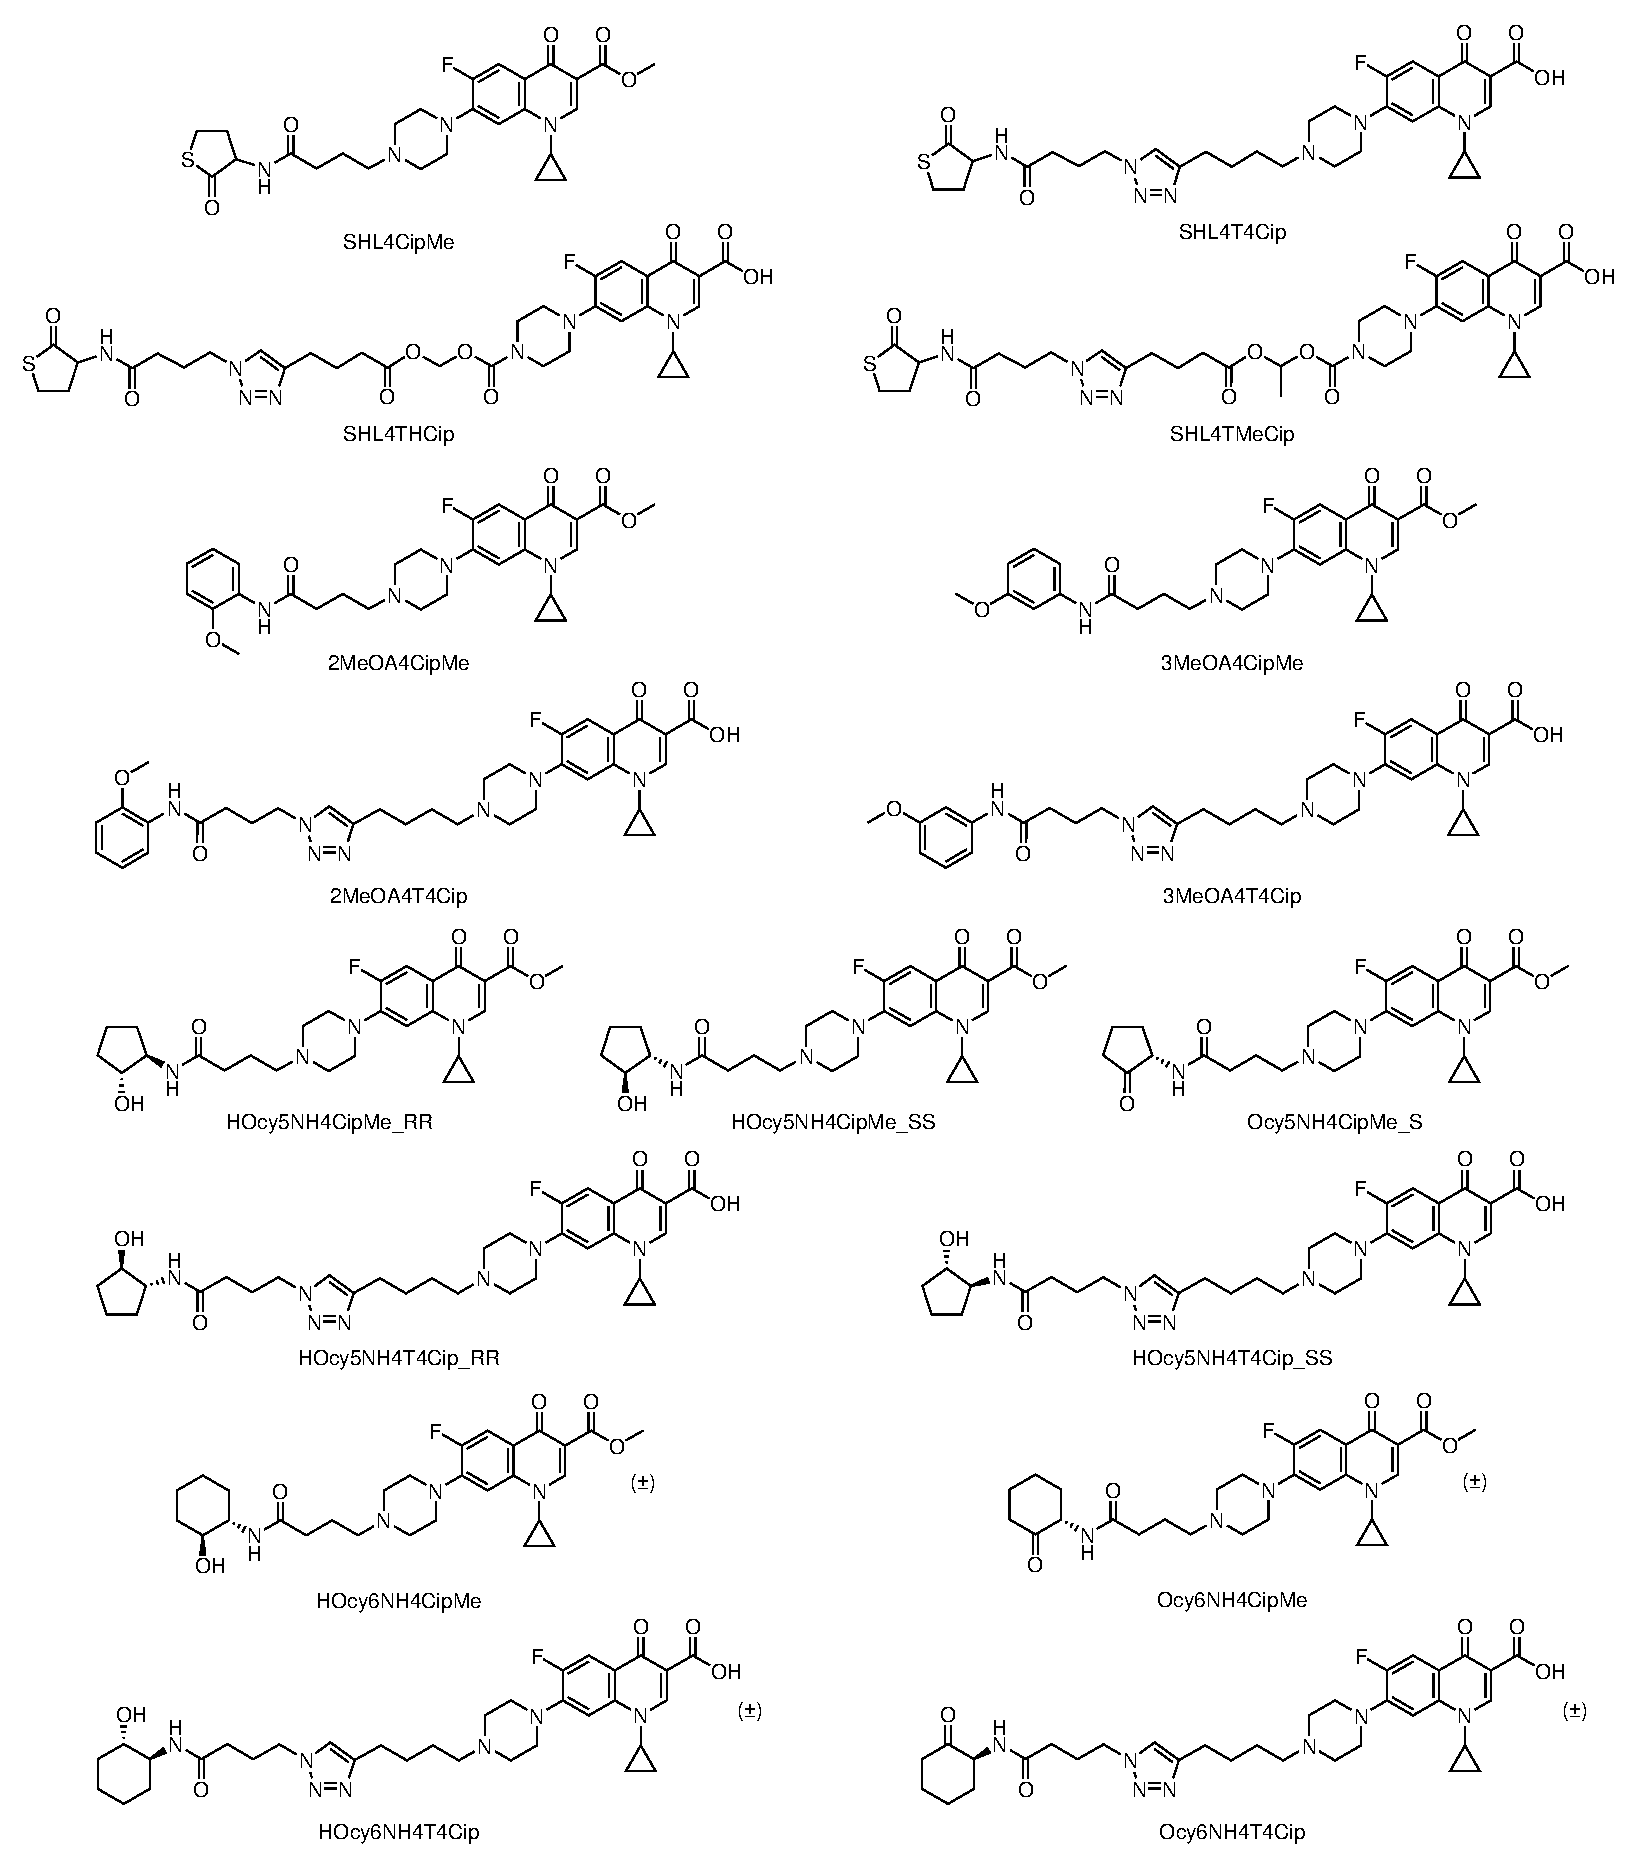
\includegraphics[scale=0.5]{finals_2}
		\caption{
 		\label{fgr:finals_2}}
	\end{center}
\end{figure}

\subsubsection{Antibacterial activity}

%The Minimum Inhibitory Concentration (MIC) is defined as the lowest concentration of an antimicrobial ingredient or agent that is bacteriostatic (prevents the visible growth of bacteria). MICs are used to evaluate the antimicrobial efficacy of various compounds by measuring the effect of decreasing concentrations of antibiotic/antiseptic over a defined period in terms of inhibition of microbial population growth.  

\subsubsubsection{YM64}

In YM64 at 5 h several of the HSL analogue-ciprofloxacin conjugates showed activity at the highest concentration (see \ref{fgr:YM64_5h_S} and \ref{fgr:YM64_5h_HO}). 
Conjugates \compound{cmpd:2MeOA4T4Cip} and \compound{cmpd:3MeOA4T4Cip} showed similar activity to ciprofloxacin \compound{cmpd:Cip} and the cleavable conjugate
\compound{cmpd:SHL4THCip} showed better activity (see \ref{fgr:YM64_5h_S}).
The activity of the cleavable conjugate \compound{cmpd:SHL4THCip} was even more pronounced at 24 h (see \ref{fgr:YM64_24h_S}).

It should be noted that the highest concentration tested was 25 $\mu$M in this set of assays as opposed to 2 $\mu$M in the previous set (see \ref{sec:bio1}), but oddly all compounds including ciprofloxacin \compound{cmpd:Cip} showed less activity. This is thought to be due to a change in the plate seals used (see \ref{sec:ABsus}). 

%trim=left bottom right top

\begin{figure}[H]
	\begin{center}
		\includegraphics[width=\textwidth,trim={1cm 1cm 1cm 1cm},clip]{"Biochem - YM64_5h_S"}
		\caption{YM64 OD readings at 5 h for the HCTL, 2-methoxybenzene and 3-methoxybenzene HSL analogue-ciprofloxacin conjugates.\label{fgr:YM64_5h_S}}
	\end{center}
\end{figure}

\begin{figure}[H]
	\begin{center}
		\includegraphics[width=\textwidth,trim={1cm 1cm 1cm 1cm},clip]{"Biochem - YM64_5h_HO"}
		\caption{YM64 OD readings at 5 h for the alcohol and ketone HSL analogue-ciprofloxacin conjugates.\label{fgr:YM64_5h_HO}}
	\end{center}
\end{figure}

\begin{figure}[H]
	\begin{center}
		\includegraphics[width=\textwidth,trim={1cm 1cm 1cm 1cm},clip]{"Biochem - YM64_24h_S"}
		\caption{YM64 OD readings at 24 h for the HCTL, 2-methoxybenzene and 3-methoxybenzene HSL analogue-ciprofloxacin conjugates.\label{fgr:YM64_24h_S}}
	\end{center}
\end{figure}

\begin{figure}[H]
	\begin{center}
		\includegraphics[width=\textwidth,trim={1cm 1cm 1cm 1cm},clip]{"Biochem - YM64_24h_HO"}
		\caption{YM64 OD readings at 24 h for the alcohol and ketone HSL analogue-ciprofloxacin conjugates.\label{fgr:YM64_24h_HO}}
	\end{center}
\end{figure}

%Growth curves for interesting ones at lowest conc compare to controls?
%9,10,11,12,15,16
%17-21,24,25
%Best 10,11,12,15,16,20,21,24,25

\subsubsubsection{PAO1}

In PAO1 at 5 h conjugates \compound{cmpd:SHL4THCip}, \compound{cmpd:2MeOA4T4Cip}, \compound{cmpd:3MeOA4T4Cip} showed activity at the highest concentration (see \ref{fgr:PAO1_5h_S}). 
The cleavable conjugate \compound{cmpd:SHL4THCip} showed similar activity to ciprofloxacin \compound{cmpd:Cip}.
At 24 h conjugate \compound{cmpd:3MeOA4T4Cip} still showed some activity, and
cleavable conjugate \compound{cmpd:SHL4THCip} showed similar activity to ciprofloxacin \compound{cmpd:Cip} (see \ref{fgr:PAO1_24h_S}).


%10,11,12,15,16,20,21,24,25 (13,14 weird)


\begin{figure}[H]
	\begin{center}
		\includegraphics[width=\textwidth,trim={1cm 1cm 1cm 1cm},clip]{"Biochem - PAO1_5h_S"}
		\caption{PAO1 OD readings at 5 h for the HCTL, 2-methoxybenzene and 3-methoxybenzene HSL analogue-ciprofloxacin conjugates.\label{fgr:PAO1_5h_S}}
	\end{center}
\end{figure}

\begin{figure}[H]
	\begin{center}
		\includegraphics[width=\textwidth,trim={1cm 1cm 1cm 1cm},clip]{"Biochem - PAO1_5h_HO"}
		\caption{PAO1 OD readings at 5 h for the alcohol and ketone HSL analogue-ciprofloxacin conjugates.\label{fgr:PAO1_5h_HO}}
	\end{center}
\end{figure}


\begin{figure}[H]
	\begin{center}
		\includegraphics[width=\textwidth,trim={1cm 1cm 1cm 1cm},clip]{"Biochem - PAO1_24h_S"}
		\caption{PAO1 OD readings at 24 h for the HCTL, 2-methoxybenzene and 3-methoxybenzene HSL analogue-ciprofloxacin conjugates.\label{fgr:PAO1_24h_S}}
	\end{center}
\end{figure}

\begin{figure}[H]
	\begin{center}
		\includegraphics[width=\textwidth,trim={1cm 1cm 1cm 1cm},clip]{"Biochem - PAO1_24h_HO"}
		\caption{PAO1 OD readings at 24 h for the alcohol and ketone HSL analogue-ciprofloxacin conjugates.\label{fgr:PAO1_24h_HO}}
	\end{center}
\end{figure}





Approximate MICs for the more active compounds are shown in \ref{tbl:MICs}

\begin{table}[H]
  \centering
\begin{tabular}{|p{0.12\textwidth}|p{0.08\textwidth}|p{0.08\textwidth}|p{0.08\textwidth}|p{0.08\textwidth}|}
\hline  
\textbf{Compound} & \textbf{YM64 - 5 h} & \textbf{YM64 - 24 h} & \textbf{PAO1 - 5 h} & \textbf{PAO1 - 24 h} \\ 
\hline 
SHL4THCip \compound{cmpd:SHL4THCip} &  &  &  & 0.0455 $\pm$ \\ 
\hline 
2MeOA4T4Cip \compound{cmpd:2MeOA4T4Cip} & 0.0406 $\pm$ & 0.0391 $\pm$ &  &  \\ 
\hline 
3MeOA4T4Cip \compound{cmpd:3MeOA4T4Cip} &  & 0.0364 $\pm$ &  &  \\ 
\hline 
Cip \compound{cmpd:Cip} &  &  &  &  \\ 
\hline
\end{tabular}
\caption{.\label{tbl:}} 
\end{table}


%\subsubsection{HGS4}
%(can't see 9-16 graphs, check)
%1-25 no inhibition
%except 11 a bit
%
%
%
%
%\subsubsection{HGS4 complemented}
%
%11,16,19,20,21,22,24,25

\subsubsection{Determination of anti-biofilm activity}

Biofilm growth was measured using crystal violet staining\cite{OToole1998}.

\subsubsection{Effect on biofilm formation}





\subsubsection{Biofilm disruption}



